\documentclass{article}
\usepackage[utf8]{inputenc}
\usepackage[spanish]{babel}
\usepackage{graphicx}
\graphicspath{ {images/} }
\usepackage{ragged2e}
\usepackage{url}


\begin{document}

\begin{titlepage}
    \begin{center}
        \vspace*{1cm}
        
        \Huge
        \textbf{Informe Parcial I}
            
        \vspace{0.5cm}
        \LARGE
       \textit{ Informática II}
            
        \vspace{1.5cm}
            
        \textbf{ESTEBAN JARAMILLO PÉREZ\\
        SANTIAGO MUÑOZ JIMÉNEZ\\
        DANIEL ALEJANDRO VALENCIA}
            
        \vfill
            
        \vspace{0.8cm}
            
        \Large
        Despartamento de Ingeniería Electrónica y Telecomunicaciones\\
        Universidad de Antioquia\\
        Medellín\\
        Febrero de 2022
            
    \end{center}
\end{titlepage}

\tableofcontents
\newpage
\newpage
\section{Objetivos de la practica(sujeto a cambios)}
\label{objetivos}
\textbf{Objetivo general}\\
Desarrollar un sistema de comunicación entre maquinas que pasen la información obtenida del usuario
\newline
\newline
\textbf{Objetivo Específicos}

\justify
\begin{itemize}

    \item utilizar el circuito integrado 74HC595 de forma independiente con pulsadores o switches.
    
    \item usar Arduino detallando la utilidad que puede darle a este elemento para la solución del problema.
    
    \item  Realizar una comunicación entre dos Arduinos usando puertos digitales

    \item Programar en QT el código de encriptación y desencriptación
    
    \item Realizar en Arduino un circuito con una pantalla LCD que muestre la información real del mensaje
    
   
    
\end{itemize}


\newpage
\section{Uso del circuito integrado 74HC595.}
\label{74HC595}


Es un Chip que permite el desplazamiento de bits en un registro, es decir, que permite el ingreso serial (un bit) de datos, para luego obtener una salida en paralelo (8 bits); dependeran de los valores de entrada en serie (3 bits) y de los que ya están almacenados.

Este sistema es conocido por su tipo de desplazamiento en serie-paralelo, que con una sola entrada se pueden controlar las ocho salidas.Este mecanismo es controlado por una señal de reloj, el cual es usado para llevar el ritmo al que trabajara.Un ejemplo claro de este dispositivo es en el uso control original de Nintendo que necesita presionar todos los botones en serie.(cada pulso de un botón, es transformado por el 595 en una salida de 8 bits).

La figura 1 presenta un proceso donde al ser aplicada una pulsación, sucede que cada bit se mueve una posición a la izquierda,por ejemplo, el bit 7 cambia al valor que estaba en el 6 y así sucesivamente.También al llevar a cabo la pulsación, el PIN DATA, llevará un registro de altos y bajos, donde el primero marcará 1’s y el segundo 0’s

Con respecto a la figura 1 el PIN “latch” es utilizado para realizar una copia del DATA(Shift Register), que cada vez que este va recibiendo información, manda esos 8 bits al latch (Storage Register), si la salida se encuentra habilitada, los bits del latch son activados en los pin de salida (Output).


\centering
\includegraphics[scale=0.5]{figura1}
imagen tomada de: https://lastminuteengineers.com/
\newpage

A continuación se mostrará el paso a paso y la utilidad que se le dio a los siguientes ejemplos.\newline


\textbf{(1)Circuito 595 con pulsador:} \\
\justify Se empleo un arduino, unas luces led, unas resistencias, un pequeño pulsador para probar el uso del reloj , la tierra (cable negro) y el positivo (cable rojo) se pegaran a la placa, sin el uso de estos dos no hara un correcto funcionamiento, ademas el uso de las salidas (cables azules) son usados para poder encender los leds, la entrada (cable verde) y el reloj de registro de desplazamiento (cable naranja) se utilizaron unidos al arduino, esto es debido a que con el uso de un pulsador, el voltaje se sobrepasaba, aunque con el uso de la bateria de 9V no era sufieciente, esto hacia que el circuito se quemara. Por otro lado, el reloj de salida, el que permite el ritmo de trabajo, es utilizado por medio de este pulsador, en este es necesario el uso de dos resistencia para llevar el control del voltaje y también el uso de un cable positivo, cada vez que se le presiona, este envía la señal y de esta forma permite llevar la información, esta es simulada con los leds encendidos.
\newline
\newline
\newline
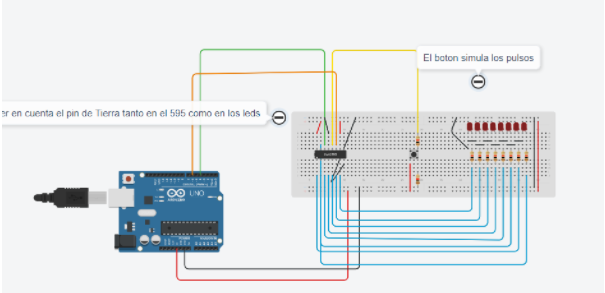
\includegraphics[scale=0.5]{figura2}
\centering
\textbf{Apoyado en el anexo 1}
\newline
\newline
\newline



\textbf{(1)Circuito 595 sin pulsador:} \\
\justify Se empleó un arduino, unas luces led, unas resistencias y una placa. La tierra (cable negro) y el positivo (cable rojo) se pegaran a la placa, sin el uso de estos dos no hara un correcto funcionamiento, ademas el uso de las salidas (cables azules) son usados para poder encender los leds, la entrada (cable verde), el reloj de registro de desplazamiento (cable naranja) y el reloj de salida(cable amarillo).Como muestra la imagen cada uno esta conectado al arduino y al 595, permitiendo un correcto funcionamiento y el voltaje adecuado, es importante tener en cuenta el lugar al que va colocado cada cable, de lo contrario podrian ocurrir errores como lo son una mala ejecucion o el daño del circuito 595..
\newline
\newline
\newline
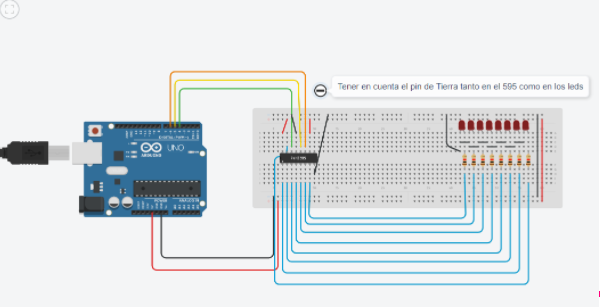
\includegraphics[scale=0.5]{figura3.png}
\centering
\textbf{Apoyado en el anexo 2}
\newline
\newline
\newline

\newpage
\justify
\section{Anexos}
\label{Anexos}
\textbf{(1)}
\url{https://www.tinkercad.com/things/6ROBFOLGDwK-copy-of-74hc595/editel?sharecode=t7hqpOIFHnGtsxOCjGsjoC3OBudnwDUmjirfRQvRiZU}
\newline
\newline
\textbf{(2)}
\url{https://www.tinkercad.com/things/6VynWWL64fP-74hc595/editel?sharecode=ot5gC80GJt7dIHeJV_Vv7UX7wF0xgc8KLDBU_-QefwY}

\newpage
\section{Referencias}
\label{Referencias}

\justify
Last Minute Engineers -. (2021). Last Minute Engineers. https://lastminuteengineers.com/
\newline
I. (2019, 18 julio). 74hc595: todo sobre el CI de registro de desplazamiento. Hardware libre. https://www.hwlibre.com/




\end{document}



